% Options for packages loaded elsewhere
\PassOptionsToPackage{unicode}{hyperref}
\PassOptionsToPackage{hyphens}{url}
\PassOptionsToPackage{dvipsnames,svgnames,x11names}{xcolor}
%
\documentclass[
]{scrartcl}

\usepackage{amsmath,amssymb}
\usepackage{iftex}
\ifPDFTeX
  \usepackage[T1]{fontenc}
  \usepackage[utf8]{inputenc}
  \usepackage{textcomp} % provide euro and other symbols
\else % if luatex or xetex
  \usepackage{unicode-math}
  \defaultfontfeatures{Scale=MatchLowercase}
  \defaultfontfeatures[\rmfamily]{Ligatures=TeX,Scale=1}
\fi
\usepackage{lmodern}
\ifPDFTeX\else  
    % xetex/luatex font selection
\fi
% Use upquote if available, for straight quotes in verbatim environments
\IfFileExists{upquote.sty}{\usepackage{upquote}}{}
\IfFileExists{microtype.sty}{% use microtype if available
  \usepackage[]{microtype}
  \UseMicrotypeSet[protrusion]{basicmath} % disable protrusion for tt fonts
}{}
\makeatletter
\@ifundefined{KOMAClassName}{% if non-KOMA class
  \IfFileExists{parskip.sty}{%
    \usepackage{parskip}
  }{% else
    \setlength{\parindent}{0pt}
    \setlength{\parskip}{6pt plus 2pt minus 1pt}}
}{% if KOMA class
  \KOMAoptions{parskip=half}}
\makeatother
\usepackage{xcolor}
\setlength{\emergencystretch}{3em} % prevent overfull lines
\setcounter{secnumdepth}{-\maxdimen} % remove section numbering
% Make \paragraph and \subparagraph free-standing
\ifx\paragraph\undefined\else
  \let\oldparagraph\paragraph
  \renewcommand{\paragraph}[1]{\oldparagraph{#1}\mbox{}}
\fi
\ifx\subparagraph\undefined\else
  \let\oldsubparagraph\subparagraph
  \renewcommand{\subparagraph}[1]{\oldsubparagraph{#1}\mbox{}}
\fi


\providecommand{\tightlist}{%
  \setlength{\itemsep}{0pt}\setlength{\parskip}{0pt}}\usepackage{longtable,booktabs,array}
\usepackage{calc} % for calculating minipage widths
% Correct order of tables after \paragraph or \subparagraph
\usepackage{etoolbox}
\makeatletter
\patchcmd\longtable{\par}{\if@noskipsec\mbox{}\fi\par}{}{}
\makeatother
% Allow footnotes in longtable head/foot
\IfFileExists{footnotehyper.sty}{\usepackage{footnotehyper}}{\usepackage{footnote}}
\makesavenoteenv{longtable}
\usepackage{graphicx}
\makeatletter
\def\maxwidth{\ifdim\Gin@nat@width>\linewidth\linewidth\else\Gin@nat@width\fi}
\def\maxheight{\ifdim\Gin@nat@height>\textheight\textheight\else\Gin@nat@height\fi}
\makeatother
% Scale images if necessary, so that they will not overflow the page
% margins by default, and it is still possible to overwrite the defaults
% using explicit options in \includegraphics[width, height, ...]{}
\setkeys{Gin}{width=\maxwidth,height=\maxheight,keepaspectratio}
% Set default figure placement to htbp
\makeatletter
\def\fps@figure{htbp}
\makeatother
\newlength{\cslhangindent}
\setlength{\cslhangindent}{1.5em}
\newlength{\csllabelwidth}
\setlength{\csllabelwidth}{3em}
\newlength{\cslentryspacingunit} % times entry-spacing
\setlength{\cslentryspacingunit}{\parskip}
\newenvironment{CSLReferences}[2] % #1 hanging-ident, #2 entry spacing
 {% don't indent paragraphs
  \setlength{\parindent}{0pt}
  % turn on hanging indent if param 1 is 1
  \ifodd #1
  \let\oldpar\par
  \def\par{\hangindent=\cslhangindent\oldpar}
  \fi
  % set entry spacing
  \setlength{\parskip}{#2\cslentryspacingunit}
 }%
 {}
\usepackage{calc}
\newcommand{\CSLBlock}[1]{#1\hfill\break}
\newcommand{\CSLLeftMargin}[1]{\parbox[t]{\csllabelwidth}{#1}}
\newcommand{\CSLRightInline}[1]{\parbox[t]{\linewidth - \csllabelwidth}{#1}\break}
\newcommand{\CSLIndent}[1]{\hspace{\cslhangindent}#1}

\usepackage{authblk}
\usepackage[version=4]{mhchem}
\makeatletter
\@ifpackageloaded{tcolorbox}{}{\usepackage[skins,breakable]{tcolorbox}}
\@ifpackageloaded{fontawesome5}{}{\usepackage{fontawesome5}}
\definecolor{quarto-callout-color}{HTML}{909090}
\definecolor{quarto-callout-note-color}{HTML}{0758E5}
\definecolor{quarto-callout-important-color}{HTML}{CC1914}
\definecolor{quarto-callout-warning-color}{HTML}{EB9113}
\definecolor{quarto-callout-tip-color}{HTML}{00A047}
\definecolor{quarto-callout-caution-color}{HTML}{FC5300}
\definecolor{quarto-callout-color-frame}{HTML}{acacac}
\definecolor{quarto-callout-note-color-frame}{HTML}{4582ec}
\definecolor{quarto-callout-important-color-frame}{HTML}{d9534f}
\definecolor{quarto-callout-warning-color-frame}{HTML}{f0ad4e}
\definecolor{quarto-callout-tip-color-frame}{HTML}{02b875}
\definecolor{quarto-callout-caution-color-frame}{HTML}{fd7e14}
\makeatother
\makeatletter
\makeatother
\makeatletter
\makeatother
\makeatletter
\@ifpackageloaded{caption}{}{\usepackage{caption}}
\AtBeginDocument{%
\ifdefined\contentsname
  \renewcommand*\contentsname{Table of contents}
\else
  \newcommand\contentsname{Table of contents}
\fi
\ifdefined\listfigurename
  \renewcommand*\listfigurename{List of Figures}
\else
  \newcommand\listfigurename{List of Figures}
\fi
\ifdefined\listtablename
  \renewcommand*\listtablename{List of Tables}
\else
  \newcommand\listtablename{List of Tables}
\fi
\ifdefined\figurename
  \renewcommand*\figurename{Figure}
\else
  \newcommand\figurename{Figure}
\fi
\ifdefined\tablename
  \renewcommand*\tablename{Table}
\else
  \newcommand\tablename{Table}
\fi
}
\@ifpackageloaded{float}{}{\usepackage{float}}
\floatstyle{ruled}
\@ifundefined{c@chapter}{\newfloat{codelisting}{h}{lop}}{\newfloat{codelisting}{h}{lop}[chapter]}
\floatname{codelisting}{Listing}
\newcommand*\listoflistings{\listof{codelisting}{List of Listings}}
\makeatother
\makeatletter
\@ifpackageloaded{caption}{}{\usepackage{caption}}
\@ifpackageloaded{subcaption}{}{\usepackage{subcaption}}
\makeatother
\makeatletter
\@ifpackageloaded{tcolorbox}{}{\usepackage[skins,breakable]{tcolorbox}}
\makeatother
\makeatletter
\@ifundefined{shadecolor}{\definecolor{shadecolor}{rgb}{.97, .97, .97}}
\makeatother
\makeatletter
\makeatother
\makeatletter
\makeatother
\makeatletter
\@ifpackageloaded{fontawesome5}{}{\usepackage{fontawesome5}}
\makeatother
\ifLuaTeX
  \usepackage{selnolig}  % disable illegal ligatures
\fi
\IfFileExists{bookmark.sty}{\usepackage{bookmark}}{\usepackage{hyperref}}
\IfFileExists{xurl.sty}{\usepackage{xurl}}{} % add URL line breaks if available
\urlstyle{same} % disable monospaced font for URLs
\hypersetup{
  pdftitle={Crash Course in Materials Science of Superconductors},
  pdfauthor={Stefan Bringuier},
  pdfkeywords={Superconductors, Materials Science},
  colorlinks=true,
  linkcolor={blue},
  filecolor={Maroon},
  citecolor={Blue},
  urlcolor={Blue},
  pdfcreator={LaTeX via pandoc}}

\title{Crash Course in Materials Science of Superconductors}

  \author{Stefan Bringuier}
          \affil{%
          Materials Scientist \\
          ORCID: \href{https://orcid.org/0000-0001-6753-1437}{0000-0001-6753-1437}\\
          \href{mailto:stefanbringuier@gmail.com}{stefanbringuier@gmail.com}\\
          \href{https://stefanbringuier.info}{https://stefanbringuier.info}
      }
    
\date{Sep 12, 2023}
\begin{document}
\maketitle
\begin{abstract}
Crash Course in Materials Science of Superconductors
\end{abstract}
\ifdefined\Shaded\renewenvironment{Shaded}{\begin{tcolorbox}[interior hidden, enhanced, frame hidden, sharp corners, borderline west={3pt}{0pt}{shadecolor}, breakable, boxrule=0pt]}{\end{tcolorbox}}\fi

\renewcommand*\contentsname{Table of contents}
{
\hypersetup{linkcolor=}
\setcounter{tocdepth}{3}
\tableofcontents
}
\listoffigures
\hypertarget{some-comments}{%
\subsection{Some Comments}\label{some-comments}}

\begin{tcolorbox}[enhanced jigsaw, opacitybacktitle=0.6, colframe=quarto-callout-important-color-frame, toptitle=1mm, arc=.35mm, toprule=.15mm, rightrule=.15mm, title=\textcolor{quarto-callout-important-color}{\faExclamation}\hspace{0.5em}{Important}, colbacktitle=quarto-callout-important-color!10!white, opacityback=0, titlerule=0mm, bottomtitle=1mm, coltitle=black, leftrule=.75mm, bottomrule=.15mm, colback=white, breakable, left=2mm]

These are working notes, so there are bound to be errors. Please keep
this in mind while going through the notes. Feel free to email
\href{mailto:stefanbringuier@gmail.com}{me} if you want to provide
corrections.

\end{tcolorbox}

\begin{tcolorbox}[enhanced jigsaw, opacitybacktitle=0.6, colframe=quarto-callout-note-color-frame, toptitle=1mm, arc=.35mm, toprule=.15mm, rightrule=.15mm, title=\textcolor{quarto-callout-note-color}{\faInfo}\hspace{0.5em}{Note}, colbacktitle=quarto-callout-note-color!10!white, opacityback=0, titlerule=0mm, bottomtitle=1mm, coltitle=black, leftrule=.75mm, bottomrule=.15mm, colback=white, breakable, left=2mm]

Much of the notes derived from monograph by Packwood and textbook by
Garnett.\textsuperscript{\textbf{Packwood:2017?},\textbf{Garnett:2023?}}

\end{tcolorbox}

\begin{tcolorbox}[enhanced jigsaw, opacitybacktitle=0.6, colframe=quarto-callout-tip-color-frame, toptitle=1mm, arc=.35mm, toprule=.15mm, rightrule=.15mm, title=\textcolor{quarto-callout-tip-color}{\faLightbulb}\hspace{0.5em}{Tip}, colbacktitle=quarto-callout-tip-color!10!white, opacityback=0, titlerule=0mm, bottomtitle=1mm, coltitle=black, leftrule=.75mm, bottomrule=.15mm, colback=white, breakable, left=2mm]

If you prefer to view this in a report format, you can download a
formatted PDF of this presentation
\href{presentation_reportformat.pdf}{here}.

\end{tcolorbox}

\hypertarget{whats-all-the-fuss}{%
\subsection{Whats all the fuss}\label{whats-all-the-fuss}}

\begin{itemize}
\tightlist
\item
  Why did anyone care to begin with?

  \begin{itemize}
  \tightlist
  \item
    They didn't. Initially Heike Kamerlingh Onnes\textsuperscript{1} and
    others were just interested in cryogenics.
  \item
    Once they achieved liquid Helium, they asked why note study
    conductive metals at these temperatures.
  \item
    In 1911 Kamerlingh Onnes started with elemental Mercury, 💥 the
    field of SC\footnote{SC: Superconductivity} was born.
  \end{itemize}
\item
  Physcist focused on measurement of other elemental solides and a
  theory.
\item
  Observation of SC in Nb begun technological use.
\end{itemize}

\begin{figure}[H]

{\centering 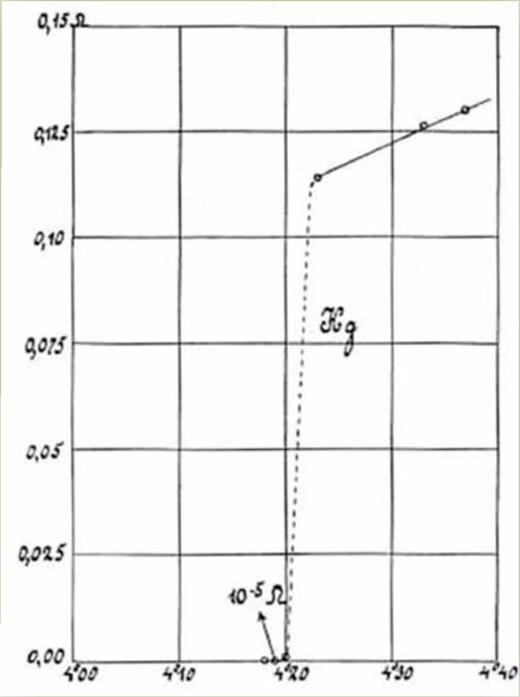
\includegraphics{../figures/HgSC_HKO.jpeg}

}

\caption{Original plot of Hg transition temperature to SC phase.}

\end{figure}

\hypertarget{backmatter}{%
\subsection{Backmatter}\label{backmatter}}

\begin{figure}[H]

{\centering 

\href{https://www.stefanbringuier.info}{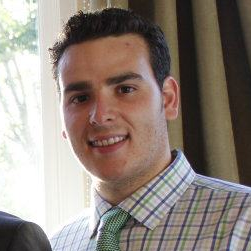
\includegraphics[width=1.30208in,height=\textheight]{figures/stefanbringuier.png}}

}

\end{figure}

\href{mailto:stefanbringuier@gmail.com}{\nolinkurl{stefanbringuier@gmail.com}}

\href{https://github.com/stefanbringuier}{\faIcon{github}}
\href{https://linkedin.com/in/stefanbringuier}{\faIcon{linkedin}}
\href{https://scholar.google.com/citations?user=MhJTimgAAAAJ\&hl=en}{}
\href{https://orcid.org/0000-0001-6753-1437}{}

\begin{tcolorbox}[enhanced jigsaw, opacitybacktitle=0.6, colframe=quarto-callout-note-color-frame, toptitle=1mm, arc=.35mm, toprule=.15mm, rightrule=.15mm, title=\textcolor{quarto-callout-note-color}{\faInfo}\hspace{0.5em}{Note}, colbacktitle=quarto-callout-note-color!10!white, opacityback=0, titlerule=0mm, bottomtitle=1mm, coltitle=black, leftrule=.75mm, bottomrule=.15mm, colback=white, breakable, left=2mm]

This presentation can be viewed online at
\url{https://stefanbringuier.github.io/BayesianOptNotes}.

To export \texttt{revealjs} presentations to pdf, press `e' then
`ctrl-p' ➡ `save as pdf'

\end{tcolorbox}

\begin{tcolorbox}[enhanced jigsaw, opacitybacktitle=0.6, colframe=quarto-callout-tip-color-frame, toptitle=1mm, arc=.35mm, toprule=.15mm, rightrule=.15mm, title=\textcolor{quarto-callout-tip-color}{\faLightbulb}\hspace{0.5em}{Tip}, colbacktitle=quarto-callout-tip-color!10!white, opacityback=0, titlerule=0mm, bottomtitle=1mm, coltitle=black, leftrule=.75mm, bottomrule=.15mm, colback=white, breakable, left=2mm]

A report formated PDF of this presentation can be downloaded
\href{presentation_reportformat.pdf}{here}.

\end{tcolorbox}

\hypertarget{references}{%
\subsection{References}\label{references}}

\hypertarget{refs}{}
\begin{CSLReferences}{0}{0}
\leavevmode\vadjust pre{\hypertarget{ref-OnnesReview2010}{}}%
\CSLLeftMargin{1. }%
\CSLRightInline{Delft, D. van \& Kes, P.
\href{https://doi.org/10.1063/1.3490499}{{The discovery of
superconductivity}}. \emph{Physics Today} \textbf{63,} 38--43 (2010).}

\leavevmode\vadjust pre{\hypertarget{ref-Speller2022}{}}%
\CSLLeftMargin{2. }%
\CSLRightInline{Speller, S. \emph{A materials science guide to
superconductors and how to make them super}. (Oxford University Press,
2022).}

\end{CSLReferences}

I. Introduction Slide 1: Title Slide Slide 2: Objectives of the
Presentation Slide 3: Overview of Topics Covered Slide 4: Importance of
Superconducting Materials Slide 5: Brief History of Superconductivity
II. Basics of Superconductivity (Theory) Slides 6-10 Cooper Pairs
Meissner Effect BCS Theory Overview Zero Electrical Resistance Critical
Temperature III. Applications: Magnetics and Wires Slides 11-15 MRI
Machines Maglev Trains Energy Grids Superconducting Coils Limitations in
Applications IV. Thermodynamics and Phases Slides 16-20 Type I and Type
II Superconductors Critical Fields Diamagnetic Response Phase Diagrams
Energy Gaps V. Flux Pinning and Levitation Slides 21-25 Vortex Lattices
Flux Tubes Levitation Applications Pinning Centers YBaCuO Examples VI.
Niobium-Titanium (NbTi) Alloys Slides 26-30 Composition and Structure
Magnetic Properties Mechanical Properties Applications Processing
Challenges VII. Quantum Effects Slides 31-35 Quantum Tunneling Josephson
Junctions Macroscopic Quantum Phenomena SQUIDs Quantum Computing
Applications VIII. Microstructure and Grain Boundaries Slides 36-40
Grain Boundary Impact on Properties Microstructure Analysis Sintering
Methods Weak Links Influence on Flux Pinning IX. Mechanical Properties
Slides 41-45 Tensile Strength Brittleness Fatigue Thermal Expansion
Composite Superconductors X. High-Temperature Superconductors (HTSC)
Slides 46-50 YBaCuO and Other Cuprates Iron-based Superconductors
Challenges and Advantages Applications Current Research Trends XI.
Recent Trends and Future Directions Slides 51-55 MgB2 Developments
Room-Temperature Superconductors Topological Superconductors
Commercialization Challenges Research Funding and Outlook XII.
Conclusion and Summary Slide 56: Summary of Key Points Slide 57: Future
Outlook Slide 58: Acknowledgments Slide 59: Questions Slide 60:
References



\end{document}
